% !TEX encoding = UTF-8 Unicode
\chapter{Marco teórico}

%En esta sección se presentarán los fundamentos teóricos sobre los cuales se basa el presente trabajo. 
%\sout{También se hablará} \textcolor{red}{entrada muy informal} del funcionamiento de los diferentes dispositivos que serán usados en los diferentes experimentos.

En el presente capítulo se abordarán los fundamentos teóricos sobre los cuales se basa el presente trabajo.
Además, se proporcionará información acerca del funcionamiento de los diferentes dispositivos utilizados en las pruebas experimentales.

\section{Análisis de Señales}

Una señal es todo aquello que porta información y que puede viajar a través de un medio. 
Existen dos tipos principales en los que se dividen las señales; señales discretas y señales continuas. 
Matemáticamente, las señales discretas se caracterizan por estar definidas solamente para un conjunto finito de valores de la variable independiente de una señal (normalmente la variable independiente de una señal es el tiempo y la variable dependiente corresponde a la información que porta dicha señal).
En la práctica estas señales suelen provenir de un muestreo periódico de una señal analógica.
Por otro lado, las señales continuas son señales cuyo dominio se encuentra en el conjunto de los números reales y pueden expresarse como una función matemática. 

En este trabajo, se analizarán las señales provenientes del movimiento de un vehículo, las cuales son captadas por un sensor y registradas en una computadora. 
La información de estas señales solo es captada en ciertos instantes en el tiempo, por lo cual pertenecen a la categoría de señales discretas.

En el análisis de señales es de mucha utilidad poder representar una función o señal en términos de una combinación lineal de funciones base. 
Las cuales pueden ser escogidas arbitrariamente; a condición de que estas sean ortogonales. 
Algunas de las funciones ortogonales más utilizadas en el análisis de señales son las siguientes:

\begin{itemize}
\item Funciones seno y coseno
\item Polinomios de Legendre
\item Funciones exponenciales
\item Funciones de Bessel
\item Funciones de Walsh
\item Funciones Ondeletas (Wavelets)
\end{itemize}

En este proyecto solo se hará uso de las funciones seno y coseno para representar las señales obtenidas por el sensor de aceleración. Esto debido a que mediante estas funciones es posible desintegrar de manera sencilla a la señal original, identificando los espectros de frecuencias que la componen.
%\textcolor{blue}{Esto debido a que en la práctica, los valores de aceleración de un automóvil en un intervalo de tiempo finito, siempre son acotados por un valor máximo y uno mínimo, tal y como sucede con las funciones mencionadas.
%Además de que los comportamientos en la aceleración de un vehículo que son de interés para este trabajo, consisten en aumentos y disminuciones de esta de manera recurrente, lo cual en muchas ocasiones se asemeja a un comportamiento oscilatorio.}\textcolor{red}{debes decir porqué}

\section{Análisis de Fourier}

El análisis de Fourier es usado comúnmente en el análisis de señales, principalmente para identificar las frecuencias que componen una señal o función continua \cite{Fourier}, basándose en la siguiente definición:\\

Cualquier función periódica de periodo $T$, continua por tramos e integrable sobre cualquier intervalo se puede descomponer en una suma de funciones base $seno$ y $coseno$ de la siguiente forma:\\

\begin{equation}\label{equation1}
f(t)\approx c+ \nsum[2]_{n=1}^{m}\ a_{n}\cos{\left( 2\pi nt\over T\right) } + b_{n}\sin{\left( 2\pi nt\over T\right) }
\end{equation}\\

\noindent en donde $a_{n}$ y $b_{n}$ son coeficientes que se determinan a partir de la información de la función $f(t)$ de la siguiente manera:\\

$$a_{n}={2\over T}\int_{-T\over 2}^{T\over 2} f(t)\cos{\left( 2\pi nt\over T\right) }dt$$\\

$$b_{n}={2\over T}\int_{-T\over 2}^{T\over 2} f(t)\sin{\left( 2\pi nt\over T\right) }dt$$\\

El límite $m$ de la sumatoria es un tanto arbitrario; este depende del número de términos que se deseen incluir en la sumatoria para aproximarse a la función $f(t)$. 
Entre más coeficientes se calculen e incluyan en la sumatoria, menor será la diferencia entre la función $f(t)$ y la aproximación dada por la ecuación \ref{equation1}.

La constante $c$ es un valor correspondiente a un desplazamiento de la función $f(t)$ cuyo valor queda determinado evaluando el término de la sumatoria correspondiente a $n=0$.

Entonces, en base a lo anterior, se confirma que cualquier función periódica continua se puede expresar como una mezcla de funciones base periódicas de distintas frecuencias; en este caso senos y cosenos. 
%\textcolor{orange}{esto es el teorema ¿no? entonces ya solo faltaría confirmarlo o quitarlo}

Las ecuaciones anteriores también se pueden aplicar a funciones no periódicas finitas. 
Lo que se debe de hacer en ese caso es simplemente tratar a la función como si fuese periódica; es decir, idealmente repetir indefinidamente el periodo de la función y aplicar el análisis de Fourier como si se tratase de una función periódica. 
Después de realizar el análisis, se define el dominio de las funciones base de interés en el espacio correspondiente a solo un periodo de la función.

\subsection{Caso discreto}

Es relativamente sencillo extender este análisis, de modo que también se pueda aplicar a funciones discretas, tanto periódicas como no periódicas. 
Los conceptos principales para este caso no difieren mucho de los del caso continuo. 
De igual manera al caso continuo, para el caso discreto se pretende identificar los coeficientes de las funciones base (senos y cosenos), que componen una función o señal discreta.
%En este análisis se pretende identificar los coeficientes de las funciones base (senos y cosenos) que componen una función o señal discreta. \textcolor{red}{cual es este análisis} . 
Dichas funciones base serán continuas, pero al ser sumadas tendrán que pasar por cada uno de los puntos de la función discreta que se va a analizar, lo que matemáticamente se puede expresar como:\\

$$f(t_{k})=c+ \nsum[2]_{n=1}^{N-1}\ a_{n}\cos{\left( 2\pi nt_{k}\over T\right) } + b_{n}\sin{\left( 2\pi nt_{k}\over T\right) }$$\\

\noindent en donde $N$ es el número de datos de la función $f(t_{k})$ (o de un periodo de esta, en caso de ser periódica), donde $k$ va desde $0$ hasta $N-1$.  
Donde $c$ se obtiene de manera análoga al caso continuo; $a_{n}$ y $b_{n}$ se obtienen de la siguiente manera:\\

\begin{equation}\label{equation2}
a_{n}={1\over N}\mathlarger{\mathlarger{\sum}}_{k=0}^{N-1}\ f(t_{k})\cos{\left( 2\pi nt_{k}\over T\right) }
\end{equation}\\

\begin{equation}\label{equation3}
b_{n}={1\over N}\mathlarger{\mathlarger{\sum}}_{k=0}^{N-1}\ f(t_{k})\sin{\left( 2\pi nt_{k}\over T\right) }
\end{equation}\\



Entonces, según lo anterior, se puede interpretar una función discreta como una suma de funciones armónicas seno y coseno con frecuencias y amplitudes diferentes.

Una condición importante de esta teoría es que la separación de los puntos en el dominio tiene que ser siempre la misma. 
Es decir, que la separación entre $t_k$ y $t_{k+1}$ siempre debe ser un valor constante $\Delta t$.
Esto para facilitar el álgebra de los procedimientos involucrados para llegar a las ecuaciones \ref{equation2} y \ref{equation3}.

La frecuencia más alta que se puede evaluar en las funciones armónicas está relacionada con el intervalo de separación de los datos en el dominio de la siguiente manera:\\

$$\omega_{max}={\pi \over \Delta t}$$\\

\noindent donde $\Delta t$ es la separación entre dos puntos consecutivos en el eje del dominio; usualmente es un intervalo de tiempo que separa la obtención de dos datos consecutivos de alguna señal o fuente de información.

Cabe destacar que, si el fenómeno que se está analizando presenta frecuencias mayores a la anterior, entonces el análisis realizado será erróneo, en mayor o menor medida. 
Debido a que los datos provenientes de las frecuencias mayores a $\omega_{max}$ serán incluidos como información de frecuencias menores o iguales a $\omega_{max}$. 
Lo cual es incorrecto y lo único que causará, será perturbar el análisis de la información proveniente de frecuencias que si se encuentren dentro del rango analizable. 
La solución a esto es reducir la frecuencia de muestreo $\Delta t$, hasta que $\omega_{max}$ sea mayor o igual que la frecuencia más alta involucrada en el fenómeno que se deseé analizar.

Ya que en este trabajo se analiza una señal discreta, se utilizará el análisis de Fourier para el caso discreto. 
Mediante la información proporcionada por los coeficientes $a_{n}$ y $b_{n}$ se conocerá que frecuencias están involucradas, en mayor o menor medida, en los datos obtenidos.

\section{Transformada Rápida de Fourier}
%\textcolor{blue}{
Existe una forma de calcular los coeficientes $a_{n}$ y $b_{n}$, mediante una implementación específica de la Transformada Discreta de Fourier (la cual se presentará más adelante) llamada Transformada Rápida de Fourier (o FFT por sus siglas en inglés). 
La cual consiste en un algoritmo con la función de calcular el espectro de frecuencias de una señal discreta. Cuya implementación en un equipo de cómputo es más eficiente que la forma habitual de calcular la transformada de Fourier para una señal discreta.
%}
%Existe una forma de implementar la transformada de Fourier para el caso discreto, la cual consiste en un algoritmo con la función de calcular el espectro de frecuencias de una señal discreta. Cuya implementación en un equipo de cómputo es más eficiente que la forma habitual de calcular la transformada de Fourier para una señal discreta. %\textcolor{orange}{si bien tienes un punto y coma que separa la oración la siento muy larga ve si puedes fracionarla}
Sin embargo, este método impone restricciones a cambio de la rapidez en los cálculos de la transformada, como lo es el que la cantidad de datos de la señal sea siempre una potencia de dos. 
Esto restringe un poco la cantidad de muestras útiles para la aplicación del análisis de Fourier, obligando a casi siempre tener que recortar los datos que se vayan a analizar. 
Sumado a lo anterior, este método exige la restricción de cualquier transformada discreta de Fourier, en la que el intervalo de muestreo debe ser siempre el mismo.

La Transformada Discreta de Fourier (DFT, por sus siglas en inglés) tiene una complejidad cuadrática, representada por $O(N^{2})$. 
Esto es, que el número mínimo de cálculos necesarios para obtener la información de la transformada discreta de Fourier de una señal depende cuadráticamente del número de datos de dicha señal. 
Lo cual está estrechamente relacionado con el tiempo de procesamiento empleado para realizar los cálculos necesarios de la transformada, para una señal de $N$ datos. 
Por su parte la Transformada Rápida de Fourier, con una complejidad de $O(NlogN)$, es más eficiente en cuestiones de rapidez, aunque con la desventaja de las restricciones antes mencionadas.

A continuación se da una breve descripción del funcionamiento de la transformada rápida de Fourier:

Para el caso discreto se tiene que la señal $f(t_{k})$ tiene la siguiente forma (se ha incluido al término $c$ dentro de la sumatoria):\\

\begin{equation}\label{equation4}
f(t_{k})=\mathlarger{\mathlarger{\sum}}_{n=0}^{N-1}\ a_{n}\cos{\left( \omega_{n}t_{k}\right) } + b_{n}\sin{\left( \omega_{n}t_{k}\right) }
\end{equation}\\

\noindent en donde:\\

$$\omega_{n}={2\pi n\over T} \hspace{2cm} {\rm y} \hspace{2cm} t_{k}={kT\over N}$$\\

%\textcolor{blue}{
Del análisis de Fourier para el caso discreto, se sabe que los coeficientes $a_{n}$ y $b_{n}$ se calculan de la siguiente manera:
%}\\
%De la transformada discreta de Fourier \textcolor{orange}{poner abreviación o ya sin mayúsculas} sabemos que los coeficientes $a_{n}$ y $b_{n}$ se calculan de la siguiente manera:\\

\begin{equation}\label{equation5}
a_{n}={1\over N}\mathlarger{\mathlarger{\sum}}_{k=0}^{N-1}\ f\left(t_{k}\right)\cos{\left( \omega_{n}t_{k}\right) }
\end{equation}\\

\begin{equation}\label{equation6}
b_{n}={1\over N}\mathlarger{\mathlarger{\sum}}_{k=0}^{N-1}\ f\left(t_{k}\right)\sin{\left( \omega_{n}t_{k}\right) }
\end{equation}\\

Con el fin de facilitar los cálculos del algoritmo, se expresa la ecuación \ref{equation4} en su forma exponencial compleja de la siguiente manera:\\

$$f(t_{k})=\nsum[2]_{n=0}^{N-1}\ a_{n} {{e^{i\omega_{n} t_{k}} + e^{-i\omega_{n} t_{k}}}\over 2} + b_{n} {{e^{i\omega_{n} t_{k}} - e^{-i\omega_{n} t_{k}}}\over 2i}$$\\

\noindent y reagrupando términos:\\

\begin{equation}\label{equation7}
f(t_{k})=\nsum[2]_{n=0}^{N-1}\ {1\over 2}\left(a_{n}+{b_{n}\over i}\right)e^{i\omega_{n} t_{k}} + {1\over 2}\left(a_{n}-{b_{n}\over i}\right)e^{-i\omega_{n} t_{k}}
\end{equation}\\

En este paso es importante darse cuenta de la simetría de esta ecuación, la cual puede ser aprovechada para expresarla de una manera más compacta.

Por las propiedades de paridad de las funciones seno y coseno podemos afirmar que:\\

\begin{equation}\label{equation8}
a_{n}=a_{-n}
\end{equation}

\begin{equation}\label{equation9}
-b_{n}=b_{-n}
\end{equation}\\

Además:\\

\begin{equation}\label{equation10}
e^{-i\omega_{n} t_{k}} = e^{i\omega_{-n} t_{k}}
\end{equation}\\

Aplicando las ecuaciones \ref{equation8}, \ref{equation9} y \ref{equation10} a la ecuación \ref{equation7}:\\

\begin{equation}\label{equation11}
f(t_{k})=\nsum[2]_{n=0}^{N-1}\ {1\over 2}\left(a_{n}+{b_{n}\over i}\right)e^{i\omega_{n}t_{k}} + {1\over 2}\left(a_{-n}+{b_{-n}\over i}\right)e^{i\omega_{-n}t_{k}}
\end{equation}\\

Ahora, mediante la propiedad\\

$$e^{i2\pi\left( N-n \right) t_{k}}=e^{i2\pi\left( -n \right) t_{k}}$$\\

se puede afirmar que:\\

$$\mathlarger{\mathlarger{\sum}}_{N\over 2}^{N-1}\ e^{i\omega_{n}t_{k}}=\mathlarger{\mathlarger{\sum}}_{-{N\over 2}}^{-1}\ e^{i\omega_{n}t_{k}}$$\\

Reescribiendo la ecuación \ref{equation11} usando esta propiedad:\\

\begin{equation}\label{equation12}
f(t_{k})=\nsum[2]_{-{N\over 2}}^{{N\over 2}-1}\ {1\over 2}\left(a_{n}+{b_{n}\over i}\right)e^{i\omega_{n}t_{k}} + {1\over 2}\left(a_{-n}+{b_{-n}\over i}\right)e^{i\omega_{-n}t_{k}}
\end{equation}\\

Se puede notar que la sumatoria del miembro con subíndices $n$ contiene exactamente los mismos términos que la sumatoria del miembro con subíndices $-n$. 
Por lo que ambos miembros se pueden expresar como uno solo. 
Y ya que los límites de la sumatoria de la ecuación \ref{equation12} únicamente se usaron para resaltar la simetría de la expresión, se volverá a los límites previamente establecidos, los cuales serán de utilidad en la explicación del proceso del algoritmo.
Por lo tanto, se puede expresar a la ecuación \ref{equation12} de la siguiente manera:
\\

\begin{equation}\label{equation13}
f(t_{k})=\mathlarger{\mathlarger{\sum}}_{n=0}^{N-1}\ C_{n}e^{i\omega_{n}t_{k}}
\end{equation}\\

\noindent donde\\

\begin{equation}\label{equation14}
C_{n}=a_{n}+{b_{n}\over i}={1\over N}\mathlarger{\mathlarger{\sum}}_{k=0}^{N-1}\ f(t_{k})e^{-i\omega_{n}t_{k}}
\end{equation}\\

Las ecuaciones \ref{equation14} y \ref{equation13} corresponden a la transformada discreta de Fourier y a la transformada discreta de Fourier inversa respectivamente.
Los términos $C_{n}$ son los coeficientes complejos que contienen la información de las amplitudes correspondientes al espectro de frecuencias que componen la señal $f$.

Con el fin de simplificar la explicación del algoritmo de la transformada rápida de Fourier, se usará una notación más compacta en algunos términos, como se indica a continuación:\\

$$e^{-i\omega_{n}t_{k}}\equiv x^{k}$$

$$f(t_{k})\equiv f_{k}$$\\

\noindent en donde:\\

$$x\equiv e^{-{i\omega_{n}\over N}}$$\\

El argumento empleado para desarrollar el algoritmo de la transformada rápida de Fourier parte de la división de la sumatoria de la ecuación \ref{equation14} en términos pares e impares, los cuales son incluidos en las funciones $S$ que se presentan a continuación:\\ 

$$S_{P}(x)=f_{0}+f_{2}x+\cdots+f_{N-2}x^{{N\over 2} -1}$$

$$S_{I}(x)=f_{1}+f_{3}x+\cdots+f_{N-1}x^{{N\over 2} -1}$$\\

\noindent en donde el subíndice de las funciones $S$ corresponde a los términos pares e impares.
Haciendo uso de estas funciones, se puede expresar a los coeficientes complejos $C_{n}$ de la siguiente manera:\\
%\noindent con lo cual se puede expresar a los coeficientes complejos $C_{n}$ de la siguiente manera: \textcolor{red}{evitar -> con lo cual}\\

$$C_{n}=S_{P}\left( x^{2}\right) + xS_{I}\left( x^{2}\right)$$\\

A su vez, cada una de las dos series anteriores se puede dividir igualmente en otras dos series, basándose en los términos cuya posición en la serie sea par o impar, obteniendo ahora cuatro series.\\

$$S_{P}\left( x^{2}\right)=S_{P_{21}}\left( x^{2}\right) + x^{2}S_{I_{21}}\left( x^{2}\right)$$

$$S_{I}\left( x^{2}\right)=S_{P_{22}}\left( x^{2}\right) + x^{2}S_{I_{22}}\left( x^{2}\right)$$\\

\noindent con: \\

$$S_{P_{21}}=f_{0}+f_{4}x^{2}+\cdots+f_{N-4}x^{{N\over 2} -2}$$

$$S_{I_{21}}=f_{2}+f_{6}x^{2}+\cdots+f_{N-2}x^{{N\over 2} -1}$$

$$S_{P_{22}}=f_{1}+f_{5}x^{2}+\cdots+f_{N-3}x^{{N\over 2} -2}$$

$$S_{I_{22}}=f_{3}+f_{7}x^{2}+\cdots+f_{N-1}x^{{N\over 2} -1}$$\\

\noindent donde el primer subíndice numérico de $S$ indica el número de divisiones en series pares e impares hechas para llegar al conjunto de series actual. 
Mientras que el segundo subíndice numérico sirve identificar series pares e impares provenientes de la misma serie. 
Se omiten los subíndices numéricos de las series de la primera división debido a que son los mismos para cada serie.

Para que los términos de las series impares concuerden con los de la serie original, se tiene que multiplicar por el factor de la exponencial elevado al cuadrado a cada una de las dos series impares anteriores.

Y así sucesivamente se puede dividir cada una de las series en otras dos, hasta llegar a series compuestas de dos términos; cuya última división dará como resultado dos series de un término cada una.
Cada vez que se divida una serie en dos, habrá que multiplicar a la serie de términos impares por el factor de la exponencial elevado a $2^{j-1}$, donde $j$ es el número de divisiones hechas para llegar a la serie en cuestión.

Por lo que al dividir la serie original $\log_{2}N$ veces, se obtendrán como resultado $N$ series de un solo término, que solo constarán de alguno de los $N$ valores de la señal $f$. 
Es en este punto donde comienza el proceso del algoritmo de la FFT, ya que conociendo los $N$ valores de $f$ se pueden encontrar todas las series de niveles superiores hasta llegar al valor del coeficiente $C_{n}$ en cuestión. 
Para formar las series de un nivel superior se multiplican a las $N\over 2$ series impares de la última división por un factor de $x^{N\over 2}$ y el resultado se suma con las correspondientes series pares:\\
\pagebreak
\begin{flalign*}
S_{P_{\log_{2}\left(N\over 2\right)i}}&=S_{P_{\log_{2}(N)2i-1}}\left( x^{2}\right) + x^{N\over 2}S_{I_{\log_{2}(N)2i-1}}\left( x^{2}\right) &\\
\end{flalign*}
\addtolength{\longa}{-3cm}
\begin{textblock*}{150mm}(7.5cm,4.7cm)
$$i=1,2,\cdots,{N\over 2}$$
\end{textblock*}
\vspace{-1cm}
\begin{flalign*}
S_{I_{\log_{2}\left(N\over 2\right)i}}&=S_{P_{\log_{2}(N)2i}}\left( x^{2}\right) + x^{N\over 2}S_{I_{\log_{2}(N)2i}}\left( x^{2}\right) &\\
\end{flalign*}
Una vez conformadas las series pares e impares del nivel superior, se multiplica a las nuevas series impares por un factor, ahora de $x^{N\over 4}$, y se suman con las correspondientes series pares.
%Aquí es donde el proceso se repite, ya que una vez encontradas las series pares e impares de un nivel arriba, se multiplica a las nuevas series impares por un factor, ahora de $x^{N\over 4}$, y se suman con las correspondientes series pares. \textcolor{orange}{No entiendo porque el -> Aqui es donde }
Repitiendo este procedimiento hasta llegar a una sola serie es como se encuentra el coeficiente $C_{n}$ deseado, cuyo valor será el de la serie encontrada.

El orden de los términos pares e impares para formar las parejas de la primera iteración es de suma importancia para llevar a cabo la transformada de manera correcta. 
Debe realizarse de manera que al final del proceso iterativo, en la última serie, los exponentes y subíndices $k$ de cada término $f_{k}x^{k}$ de la serie sean los mismos.

La ventaja de este método reside en la recursividad del proceso antes mencionado. 
Ya que, partiendo de la suma de pares de términos de la señal original se pueden encontrar las series pares e impares de un nivel arriba, las cuales a su vez servirán para encontrar la siguiente generación. 
Y así sucesivamente hasta llegar a los dos últimos términos que sumados darán como resultado el coeficiente buscado.

El proceso se puede acelerar aún más haciendo uso de la siguiente propiedad:\\

$$C_{{N\over 2}+n}=S_{P}\left( x^{2}\right) + e^{-{{i2\pi \left({N\over 2}+n\right)}\over N}}S_{I}\left( x^{2}\right)=S_{P}\left( x^{2}\right) - e^{-{{i2\pi n}\over N}}S_{I}\left( x^{2}\right)=S_{P}\left( x^{2}\right) - xS_{I}\left( x^{2}\right)$$\\

De la expresión anterior se puede notar que los factores de la última iteración, para los coeficientes $C_{n}$ y $C_{{N\over 2}+n}$ difieren solo en un factor de $-1$; siendo los términos exponenciales de las demás iteraciones idénticos para cada coeficiente $C_{n}$. 
Por lo que, los cálculos realizados para llegar a las dos series de la última iteración son de utilidad para calcular dos coeficientes (excepto cuando $n=0$, cuyo caso a diferencia del resto no presenta la simetría para encontrar a $C_{N\over 2}$):\\

$$C_{n}=S_{P}\left( x^{2}\right) + xS_{I}\left( x^{2}\right)$$

$$C_{{N\over 2}+n}=S_{P}\left( x^{2}\right) - xS_{I}\left( x^{2}\right)$$\\

Hasta este punto, basta con recorrer el índice $n$ desde 0 hasta ${N\over 2}$ para obtener el conjunto de coeficientes complejos correspondientes a la señal de $N$ datos en cuestión. 
Sin embargo, recordando que para la mayoría de los casos cada coeficiente complejo $C_{n}$ es el conjugado de $C_{N-n}$ y viceversa, el proceso se facilita aún más; al no tener que realizar los cálculos para conocer al conjugado de determinado coeficiente. 
Por lo que con esto en mente, solo hay que recorrer el índice $n$ desde $0$ hasta $N\over 4$ para obtener el conjunto completo de coeficientes complejos.

\section{Series de Tiempo}

Debido a que el objeto de estudio de este trabajo son conjuntos de datos ordenados cronológicamente, la teoría de las series de tiempo resulta fundamental para hacer un correcto análisis de la dinámica de un vehículo.

Una serie de tiempo es un conjunto de datos, los cuales se ordenan cronológicamente para que puedan ser analizados. 
El intervalo de tiempo entre dos datos consecutivos puede ser constante o puede variar según los intereses del análisis, o la forma en la que se recopilen los datos. 

El análisis de las series de tiempo tiene como objetivo extraer información relevante a partir de la observación, el tratamiento matemático u otras técnicas, que permitan conocer características de la serie que no son evidentes a simple vista; y que puedan responder los cuestionamientos que se tengan acerca de los datos de la serie.
Usualmente se estudia a las series de tiempo con motivos de predicción de eventos.

Se puede expresar matemáticamente una serie de tiempo $X$, de forma muy general mediante la siguiente ecuación:\\

$$X=\{X_{1}, X_{2},\ldots\}$$\\

\noindent donde el subíndice de cada valor de la señal está asociado a un orden cronológico.\\

Las series de tiempo se clasifican en dos grupos principales:

\begin{itemize}
\item {\bf Estacionarias:} Las series estacionarias son estables a lo largo del tiempo y tienen como características el que su media y su varianza oscilan alrededor de un valor constante, o bien, son constantes en el tiempo.

\item {\bf No estacionarias:} En este caso tanto la media, varianza, así como otras variables, no son constantes en el tiempo ni oscilan alrededor de un valor fijo. 
Por lo que las series de tiempo de este tipo presentan una mayor dificultad para predecir eventos futuros o extrapolar eventos pasados.
\end{itemize}

El tipo de series tratadas en el presente trabajo pertenecen a la categoría de no estacionarias. 
Esto debido a que los datos involucrados en las series con las que se trabaja se recopilan a través de sensores de aceleración, los cuales dependen del comportamiento de un vehículo a lo largo del tiempo. 
Además, existe la presencia de ruido blanco en los datos, tanto de tiempo como de aceleración, debido a un error asociado a las mediciones de los acelerómetros.
Razones por las cuales las series estudiadas presentan, en muchos casos, perturbaciones producto de esto.

\subsection{Interpolación}

Una de las herramientas más útiles y más usadas para profundizar en la información de las series de tiempo es la interpolación. 
La cual es utilizada cuando se desea conocer el valor de un dato de una serie en un instante para el cual no se tiene información. 
Dicho valor puede determinarse de manera aproximada y en algunos casos de manera exacta; su ubicación puede estar, ya sea entre dos puntos de la serie, después del último punto o antes del primero (a estos dos últimos casos se les llama extrapolación pronóstica y extrapolación retrógrada respectivamente).

Hay muchas formas de realizar una interpolación o extrapolación, según sean las necesidades del análisis y las características de los datos. 
En el presente trabajo se usará la interpolación y extrapolación lineal como parte del tratamiento de los datos.

La interpolación lineal consiste en encontrar el valor de uno o varios puntos, que se encuentran sobre la línea recta que une otros dos puntos consecutivos pertenecientes a la serie de tiempo. 
La expresión matemática que permite interpolar puntos en una serie de tiempo es la siguiente:\\

$$f(t)=f(t_{a})+(t-t_{a}){f(t_{b})-f(t_{a})\over t_{b}-t_{a}} $$\\

\noindent en donde $t_{a}$ y $t_{b}$ son los tiempos en los que se obtuvieron los datos consecutivos de la serie, $f(t_{a})$ y $f(t_{b})$ son los valores de la señal correspondientes a $t_{a}$ y $t_{b}$, mientras que $t$ es el tiempo para el que se desea conocer el valor de la serie.

Cabe destacar que la expresión anterior funciona tanto para realizar interpolaciones como extrapolaciones pronósticas y retrógradas. 
En el caso de las extrapolaciones lo único que cambia es que el punto que se desea encontrar está fuera del intervalo de los dos puntos de la serie, ya sea antes o después estos.

\section{Funcionamiento de un Acelerómetro}

Debido a que el acelerómetro es la principal herramienta de medición en este proyecto, se dará una breve explicación de la forma en que funciona este dispositivo.

Hoy en día existe una gran variedad de acelerómetros disponibles con diferentes características.
Uno de los más utilizados y el que se usó en las mediciones de este trabajo, es el acelerómetro de superficie micro-mecanizada capacitiva o acelerómetro de condensador. 
El cual está presente en la gran mayoría de los dispositivos electrónicos que requieren de este tipo de sensores.

El acelerómetro de condensador consiste en una masa sísmica de dimensiones micrométricas, hecha de silicio y unida a unos muelles. 
De manera que el movimiento de esta quede restringido a una sola dirección, como se muestra en la figura \ref{figura1}.\\

%{\fontfamily{arev}\fontsize{15}{1}\selectfont{Hab una vez ...}} 

\begin{figure}[H]
\centering
\begin{tikzpicture}[thick]
  \node{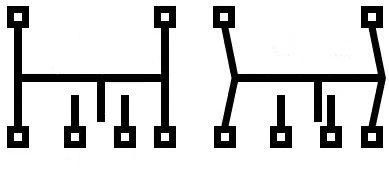
\includegraphics[scale=0.75]{mems4.jpg}};
  \node at (-3.6,1.5) {\small{\fontfamily{qhv}\selectfont Masa}};
  \node at (-2.1,1.4) {\small{\fontfamily{qhv}\selectfont Muelles}};
  \node at (3.3,1.5) {\small{\fontfamily{qhv}\selectfont Aceleración}};
  \node at (-3.6,1.1) {\small{\fontfamily{qhv}\selectfont sísmica}};
  \node at (3.3,1.1) {\small{\fontfamily{qhv}\selectfont aplicada}};
  \node at (-2.5,-2.1) {\small{\fontfamily{qhv}\selectfont Placas paralelas fijas}};
  \draw [black,-latex] (-3.6,0.85) -- (-3.6,0.55);
  \draw [black,-latex] (-1.35,1.35) -- (-0.95,1.35);
  \draw [black,-latex,line width=2pt] (2.2,1.3) -- (1.2,1.3);
  \draw [black,-latex] (-3.16,-1.9) -- (-3.16,-1.5);
  \draw [black,-latex] (-1.85,-1.9) -- (-1.85,-1.5);
\end{tikzpicture}
\caption{Esquema de un acelerómetro de condensador, también conocido como MEMS (Microelectromechanical System, por sus siglas en inglés).}
\label{figura1}
\end{figure}

Unida a la masa sísmica se encuentra una barra de silicio y colocadas a cierta distancia de la barra se encuentran dos placas fijas de dimensiones igualmente micrométricas, una a la izquierda y otra a la derecha. 
Dichas placas cumplen la misma función que un condensador de placas paralelas, de manera que cuando todo el conjunto se mueve en la dirección perpendicular a las placas, la masa sísmica y por ende la barra de silicio se moverá en dirección contraria. 
Esto causará que la distancia entre la barra y las placas cambie; provocando a su vez un cambio en el campo eléctrico generado por las placas.
Dicho cambio en el campo eléctrico también provocará un cambio en el voltaje medido, el cual, mediante otro proceso electrónico es finalmente convertido en una señal digital; que traduce el valor de este voltaje en el valor correspondiente de aceleración de la masa sísmica.\\

\section{Funcionamiento del GPS}

Durante las pruebas de conducción realizadas en este trabajo se optó por la utilización del Sistema de Posicionamiento Global (GPS, por sus siglas en inglés) para tener una mejor perspectiva de la forma de la ruta recorrida.

El GPS consta de una red de alrededor de 30 satélites orbitando alrededor de la Tierra a una altura aproximada de $20\ 000km$, con un periodo orbital de $12h$. 
Cada uno de los satélites cuenta con un reloj atómico, el cuál es indispensable para una localización precisa de los receptores en la Tierra. 
Los satélites transmiten información de su posición y tiempo actuales en intervalos de tiempo regulares. 
Las señales transmitidas por los satélites viajan a la velocidad de la luz y son interceptadas por los receptores GPS en la Tierra; los cuales calculan la distancia al satélite en base al tiempo que tardó el mensaje en llegar.

Una vez calculada la distancia del receptor GPS con un satélite, el lugar geométrico donde se puede localizar al receptor consiste en una esfera de radio igual a la distancia calculada, y cuyo centro es la posición del satélite. 
Al calcular la distancia con otro satélite se genera una segunda esfera, por lo que ahora el lugar donde se encuentra el receptor se reduce a la intersección de estas dos esferas; la cual es en la mayoría de los casos una circunferencia en el espacio. 
Intersecando dicha circunferencia con una tercera esfera, generada al medir la distancia del receptor con un tercer satélite, los lugares posibles donde se encuentra el receptor se reducen; en la gran mayoría de los casos, a dos puntos en el espacio. 
Para saber cuál de estos dos puntos es la posición real del receptor se hace una cuarta medición con otro satélite al intersecar una cuarta esfera con los dos puntos, lo cual dará como resultado un único punto cuyas coordenadas corresponden a las del receptor en la Tierra (esta última medición puede o no ser necesaria, dependiendo de las condiciones en que se realicen las primeras tres). 
El proceso anterior se ilustra en la figura \ref{figura2}.%\colorbox[rgb]{1,0,0}{(Esta explicación o la de los hiperboloides?)}\\

\begin{figure}[H]
\centering
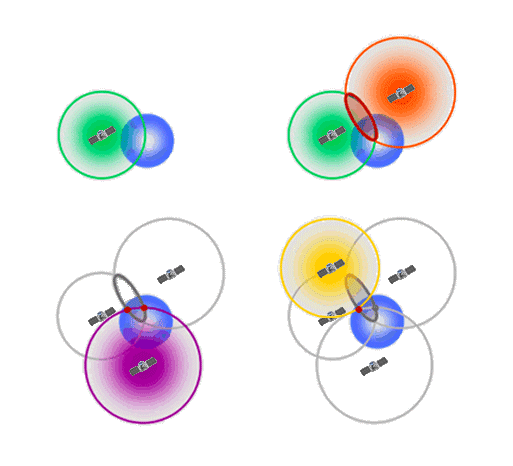
\includegraphics[scale=0.72]{GPS2.png}
\caption[Caption for LOF]{Esquema del proceso de detección de un receptor GPS en la Tierra\footnotemark[1].}
\label{figura2}
\end{figure}
\footnotetext[1]{Imagen modificada tomada de: https://wikiversus.com/deportes\text{-y-aire-libre/reloj-}gps\text{-}pulsometro/cuando-usar-glonass/}

Según el proceso explicado, se requiere en general de cuatro satélites con una línea de mira sin obstáculos hacia el receptor, para asegurar la correcta localización de este. 
Por lo general casi siempre hay más de cuatro satélites visibles para cualquier receptor en la Tierra, lo cual genera una mejor precisión en los cálculos de la posición del receptor.

\subsection{Assisted GPS}

Existe otra modalidad de esta tecnología llamada Assisted GPS (AGPS), de la cual se hizo uso en el presente trabajo.
Al igual que el GPS, el AGPS es un sistema de posicionamiento global, el cual añade nuevas metodologías para la geolocalización a las ya conocidas del GPS. 
A diferencia de los receptores GPS, que dependen únicamente de la información proporcionada por los satélites para su localización, los receptores AGPS utilizan las antenas de telefonía móvil, junto con servidores comunicados a estas, para el mismo fin. 
El uso del AGPS mejora la precisión en el proceso de localización cuando la señal emitida por los satélites es débil o existen obstáculos entre esta y los receptores. 
Otra de las ventajas que presenta este método de localización es la rapidez del proceso de localización, ya que son los servidores los encargados de recibir y almacenar en su base de datos la información correspondiente de los satélites en órbita. 
Por lo que los dispositivos con AGPS solo tienen que conectarse a estos servidores para tener dicha información a su disposición, acelerando el proceso que es llevado a cabo en un receptor GPS normal.\\

\begin{figure}[H]
\centering
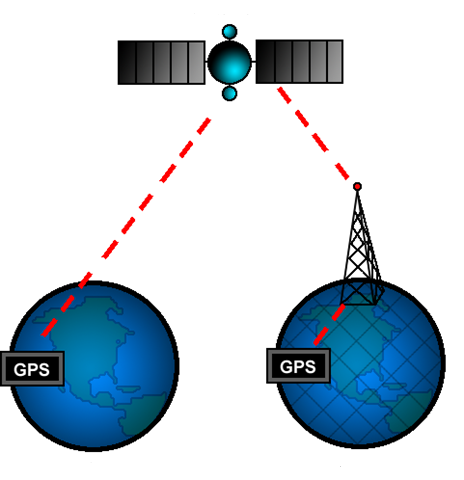
\includegraphics[scale=0.7]{a_gps2.png}
\ \\
\ \\
\caption[Caption for LOF]{Esquema de los métodos de localización por medio de GPS y de AGPS\footnotemark[1].}
\label{figura3}
\end{figure}
\footnotetext[1]{Imagen tomada de: http://www.missphones.co.uk/article/assistedgps/}
\zsavepos{sat}

\begin{textblock*}{\textwidth}(5cm,\dimexpr\paperheight-\zposy{sat}sp-105mm)
\small{\hspace{5cm} {\fontfamily{qhv}\selectfont Satélite} \\

\vspace{3cm}
\hspace{8.8cm} {\fontfamily{qhv}\selectfont Torre de}

\hspace{8.3cm} {\fontfamily{qhv}\selectfont telefonía celular}

\vspace{3.8cm}
\hspace{1.1cm} {\fontfamily{qhv}\selectfont Sistema GPS estándar} \hspace{1.3cm} {\fontfamily{qhv}\selectfont Sistema GPS asistido}}
\end{textblock*}

\section{Funcionamiento de la Tecnología Bluetooth}

La forma de almacenar los registros de aceleraciones proporcionados por el sensor se realizó mediante la transmisión inalámbrica de los datos de aceleraciones hacia un equipo de cómputo, para lo cual se decidió hacer uso de una red inalámbrica Bluetooth.

Bluetooth es un protocolo de comunicaciones para el intercambio de datos en distancias cortas, por medio de Redes Inalámbricas de Área Personal (WPAN, por sus siglas en inglés). 
La transmisión de los datos se realiza mediante radiofrecuencia, operando en un espectro de frecuencias cercano a los $2.4GHz$. 
La velocidad de transmisión de información por este medio puede alcanzar un máximo de $720kbit/s$, con un rango óptimo de $10m$.

\section{Recursos utilizados}

Para la realización y registro de las mediciones se hizo uso de diferentes dispositivos, los cuales se listan a continuación:\\

\begin{itemize}
\item {\bf Acelerómetro ADXL330.} Acelerómetro de tres ejes instalado en el mando inalámbrico Wiimote de la consola de videojuegos Wii.
\item {\bf Bluetooth.} Se utilizó la tecnología Bluetooth para la transmisión de los datos del sensor hacia un equipo de cómputo.
\item {\bf AGPS.} El AGPS fue utilizado con el fin de obtener una imagen con la cual se tuviese una mejor perspectiva de la ruta recorrida.
\end{itemize}  

\begin{figure}[H]
\centering
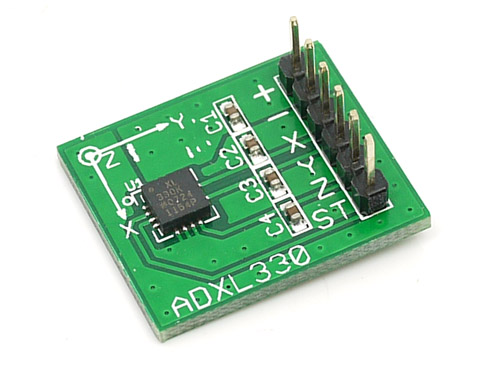
\includegraphics[scale=0.45]{adxl330v1101.jpg}
\caption[Caption for LOF]{Acelerómetro ADXL330\footnotemark[1].}
\label{figura4}
\end{figure}
\footnotetext[1]{Imagen tomada de: https://www.seeedstudio.com/Wiimote-3-Axis-Accelerometer-module-ADXL330-p-107.html}

Particularmente el mando Wiimote (figura \ref{figura5}) tiene la capacidad de detectar aceleración a lo largo de tres ejes ortogonales, mediante la utilización de el acelerómetro ADXL330 (figura \ref{figura4}). 
Tiene un promedio de frecuencia de muestreo de datos de $200Hz$, los cuales transmite a través de tecnología Bluetooth. 
Sus dimensiones son de $145mm \times 36mm \times 30mm$.
El acelerómetro ADXL330 puede percibir aceleración en un rango de $-3g$ a $3g$, donde $g$ es la aceleración debida a la fuerza de gravedad ($\approx {9.81m/s^{2}}$). 
Tiene una sensibilidad del $10\%$ y posee unas dimensiones de $4mm \times 4mm \times 1.45mm$.\\

\begin{figure}[H]
\centering
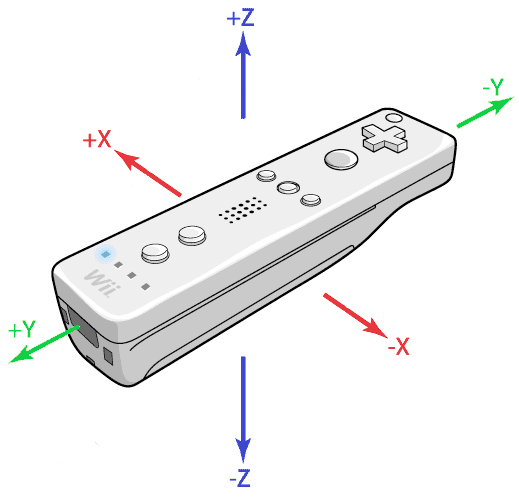
\includegraphics[scale=0.65]{wiimote2.png}
\caption[Caption for LOF]{Wiimote\footnotemark[1].}
\label{figura5}
\end{figure}
\footnotetext[1]{Imagen modificada tomada de: https://leicesterraspberrypi.wordpress.com/physics-with-a-wiimote/}

\section{Teoría del Ruido}

Muchos de los dispositivos electrónicos de medición presentan cierto grado de inexactitud en sus mediciones, lo que comúnmente se conoce como ruido.
Los dispositivos utilizados para los propósitos de este trabajo no son la excepción, por lo cual se dará una breve explicación de algunos de los diferentes tipos de ruido existentes\footnotemark[7], haciendo especial énfasis en el tipo ruido presente en las mediciones de los dispositivos utilizados.
\footnotetext[7]{Fuente: https://en.wikipedia.org/wiki/Noise{\_}(signal{\_}processing)}

En el procesamiento de señales, {\em ruido} es un término utilizado para referirse a las modificaciones no deseadas que una señal puede sufrir durante su captura, almacenamiento, transmisión, procesamiento o conversión.

El término también es usado para referirse a señales aleatorias o impredecibles que no contienen información útil, y que pueden estar o no interfiriendo con otras señales.
En la práctica, las fuentes de ruido en los diferentes tipos de señales son muy variadas; estas se clasifican en dos grupos: las fuentes de ruido externas, provenientes de la naturaleza y de los seres humanos; y las fuentes de ruido internas, las cuales son inherentes al dispositivo de medición. 

A continuación se mencionan algunos de los diferentes tipos de ruido junto con una breve explicación de cada uno.

\begin{itemize}

\item {\bf Ruido Aditivo:} Es un modelo básico de ruido, utilizado en la teoría de la información para simular el efecto de varios procesos aleatorios que ocurren en la naturaleza.
Es utilizado en medios de comunicación satelitales y espaciales. 
También es aplicado en la simulación de ruido de fondo de un canal de comunicación en estudio.

\item {\bf Ruido Blanco:} Es una señal aleatoria de cierta intensidad en una extensa gama de frecuencias, por lo que se le atribuye una densidad espectral de potencia constante. 
Este modelo toma su nombre de la luz blanca (aunque esta generalmente no tiene una densidad espectral de potencia constante en la zona de frecuencias visible). 
Es comúnmente conocido como {\em estática} y un ejemplo notable es la {\em Radiación Cósmica de Fondo}.

Este tipo de ruido se encuentra presente en el sensor utilizado para obtener datos de aceleración de un vehículo. 
Por lo cual, el ruido blanco presente en los datos obtenidos tiene la característica de ser una señal discreta, cuyas muestras son consideradas como una serie de variables aleatorias sin relación, con promedio cero y varianza finita.

Este tipo de ruido hace que el sensor tenga un margen de error de $\pm 5\%$.

\item {\bf Ruido Rosa:} Es una señal con un espectro de frecuencias tal que su densidad espectral de potencia es inversamente proporcional a la frecuencia de la señal.
El nombre proviene de la apariencia de la luz visible con este espectro de potencia.
Este tipo de ruido se presenta en fenómenos de la actividad humana como la música, imágenes artísticas, señales vitales, fluctuaciones en la economía, etc.

\item {\bf Ruido Gaussiano:} Es el tipo de ruido que presenta una función de densidad de probabilidad igual a la de una distribución Gaussiana. 
Esto quiere decir que los valores que las variables de ruido pueden tomar se encuentran en una distribución Gaussiana.
Este tipo de ruido proviene de fuentes naturales como vibraciones de átomos en conductores, radiación de cuerpo negro de la Tierra y otros objetos calientes como cuerpos celestes, entre otros.

\item {\bf Ruido Browniano:} El ruido Browniano, también conocido como ruido rojo, es el tipo de señal de ruido producida por el movimiento Browniano.
Su densidad espectral de potencia es inversamente proporcional a su frecuencia al cuadrado, lo que significa que presenta mayor energía a frecuencias bajas.
Una de las características de este tipo de ruido es que su derivada corresponde al ruido blanco.

\item {\bf Ruido Multiplicativo:} El ruido multiplicativo se refiere a un tipo de señal aleatoria que se multiplica dentro de otra señal de interés durante su captura, transmisión u otro proceso.
Un ejemplo de este tipo de ruido es el efecto de sombras producidas en fotografías digitales. 
Tal efecto se debe a ondulaciones en la superficie del objeto capturado o bien a objetos complejos presentes en la imagen, tales como follaje.

\item {\bf Ruido de Poisson:} El ruido de Poisson (conocido también como ruido de disparo) es un tipo de ruido electrónico que puede ser modelado mediante la distribución de Poisson. 
En dispositivos electrónicos, este tipo de ruido se origina a causa de la naturaleza discreta de la carga eléctrica y de la luz.
En circuitos electrónicos, consiste en fluctuaciones aleatorias de corriente eléctrica en una corriente directa.
Solo es relevante para valores pequeños de corriente eléctrica y de tiempo; ya que en una corriente eléctrica {\em común} el número de electrones que fluctúan por unidad de tiempo es muy pequeño en relación al número de electrones que no lo hacen. 
Algo similar al caso de los electrones ocurre con los fotones en haz de luz.
Entre los ámbitos en los que se presenta el ruido de Poisson se encuentran la electrónica, telecomunicaciones, detección óptica y la física fundamental.

\item {\bf Ruido Ráfaga:} Es un tipo de ruido electrónico que ocurre en semiconductores. 
Consiste en transiciones repentinas de tipo escalón entre dos o más niveles discretos de corriente o voltaje, del orden de cientos de microvolts.
Este fenómeno ocurre de manera aleatoria e impredecible y cada variación en la corriente o voltaje usualmente dura desde algunos milisegundos hasta segundos; su sonido característico es parecido a las explosiones de palomitas de maíz. 

\end{itemize}

A lo largo de este capítulo se han presentado los elementos, tanto teóricos como prácticos, necesarios para llevar a cabo los objetivos planteados.
En la siguiente sección se detallará el procedimiento realizado para obtener la información necesaria para el análisis propuesto, para lo cual se requirió del uso de los dispositivos aquí presentados.

